% !TeX root = ../thuthesis-example.tex

\chapter{相关工作}
\label{cha:related-work}

\section{三维医学模型重建}

在颅颌面手术规划及其效果预测的领域内,精确模拟术后软组织的变化至关重要。
这一过程的基础在于能够详尽表达解剖细节的面部软组织模型。
传统的计算机图形学方法,比如边界表示法(例如三角形网格)和体积表示法(例如四面体网格),被广泛用于描述实体物体的几何形态。
然而,诸如计算机断层扫描(CT)之类的医学成像技术获取的是结构化的体素数据,这种格式的数据不适合直接应用于手术模拟与效果评估。
因此,为了确保获得的数据充分符合后续处理阶段的要求,适当的数据预处理步骤变得极为重要。
这些步骤包括转换和优化原始数据集,生成适合用于外科手术模拟计算的输入模型,以增强手术规划的准确性和效果预测的可靠性。

Amberg 等研究者 \cite{ambergOptimalStepNonrigid2007} 在传统的迭代最近点(Iterative Closest Point,ICP)算法的基础上进行了扩展,提出了一种非刚性配准的方法,并维持了 ICP 算法固有的收敛特性。
这一方法的创新在于,它结合了多项正则化手段,通过不断降低刚度权重并迭代求解,有效完成了模板模型向目标几何形状的渐进逼近,实现了全局与局部形状的精细重建。
Amberg 等人工作中的一个关键创新点是利用局部仿射变换,为每个网格顶点分配了一个仿射变换,并通过施加顶点间变换差异的约束来实现稳健的配准。
此方法在多种不同类型的数据集上都表现出卓越的配准精度。

在计算机图形学领域,物体形状的表征主要依赖于边界表示法(boundary representation),其中三角形网格作为一种通用的结构已被广泛使用。
不过,显式体积表示方式如四面体网格在动画制作、物理模拟等多种任务中,因其更贴近真实世界的特性而更能够提高结果的准确程度。
鉴于此,Hang Si \cite{siTetGenDelaunaybasedQuality2015} 开发出了 TetGen 软件,用于生成高质量的四面体网格。
这一工具为数值分析和科学计算提供了卓越的基础设施。
TetGen 以 Delaunay 分割算法为核心,确保了其在理论上的正确性。
实验结果表明,TetGen 适用于处理多种复杂的三维几何体,并在实践中展现出卓越的处理效率。

理想状态下,生成的四面体网格应该准确地包含(即完美嵌入)所提供的边界面。
然而,实际模型通常由于包含自相交、非流形拓扑和开放边界等问题,难以满足 TetGen 的输入要求,这是传统网格分割方法所难以解决的挑战。
为解决这些问题,Jacobson 等研究者 \cite{jacobsonRobustInsideoutsideSegmentation2013} 提出了一种稳健的自动算法,旨在解决前述所有挑战,实现对输入模型的内部体积的精确离散化。
该算法仅要求输入的三角形网格保证外法向方向的基本一致。
通过将缠绕数(winding number)概念拓展到任意三角形网格,该算法定义了一个可用于输入模型的划分函数。
当面对封闭的三角形网格时,该函数能实现模型的理想划分,即使是对于存在众多缺陷的几何形状,算法依旧能展现出杰出的性能。该划分函数指导带约束的Delaunay分割(Constrained Delaunay Tessellation,CDT)过程,确保最终结果满足输入边界的需求。

在最近的一项研究中,Zhang Xiaoyan 等学者 \cite{zhangEFacetemplateMethodEfficiently2016} 提出了一种创新的 eFace-Template 半自动化技术,用于高效而精确地重建特定患者的面部软组织三维模型。
eFace-Template 的框架如图 \ref{fig:zhangEFacetemplateMethodEfficiently2016} 所示,此项技术的创新点在于使用了一个包含解剖学细节的模板模型,并将该模板变形至与目标几何形状相匹配,从而得到患者面部软组织的体积模型。
处理流程融合了标记驱动的混合形状变形与稠密表面配准方法,并应用了薄板样条(Thin Plate Spline,TPS)的插值方式以增强模型的泛化能力。
该方法在模型的重建精度、解剖学的准确性以及网格质量等方面都达到了较高水平。

\begin{figure}
  \centering
  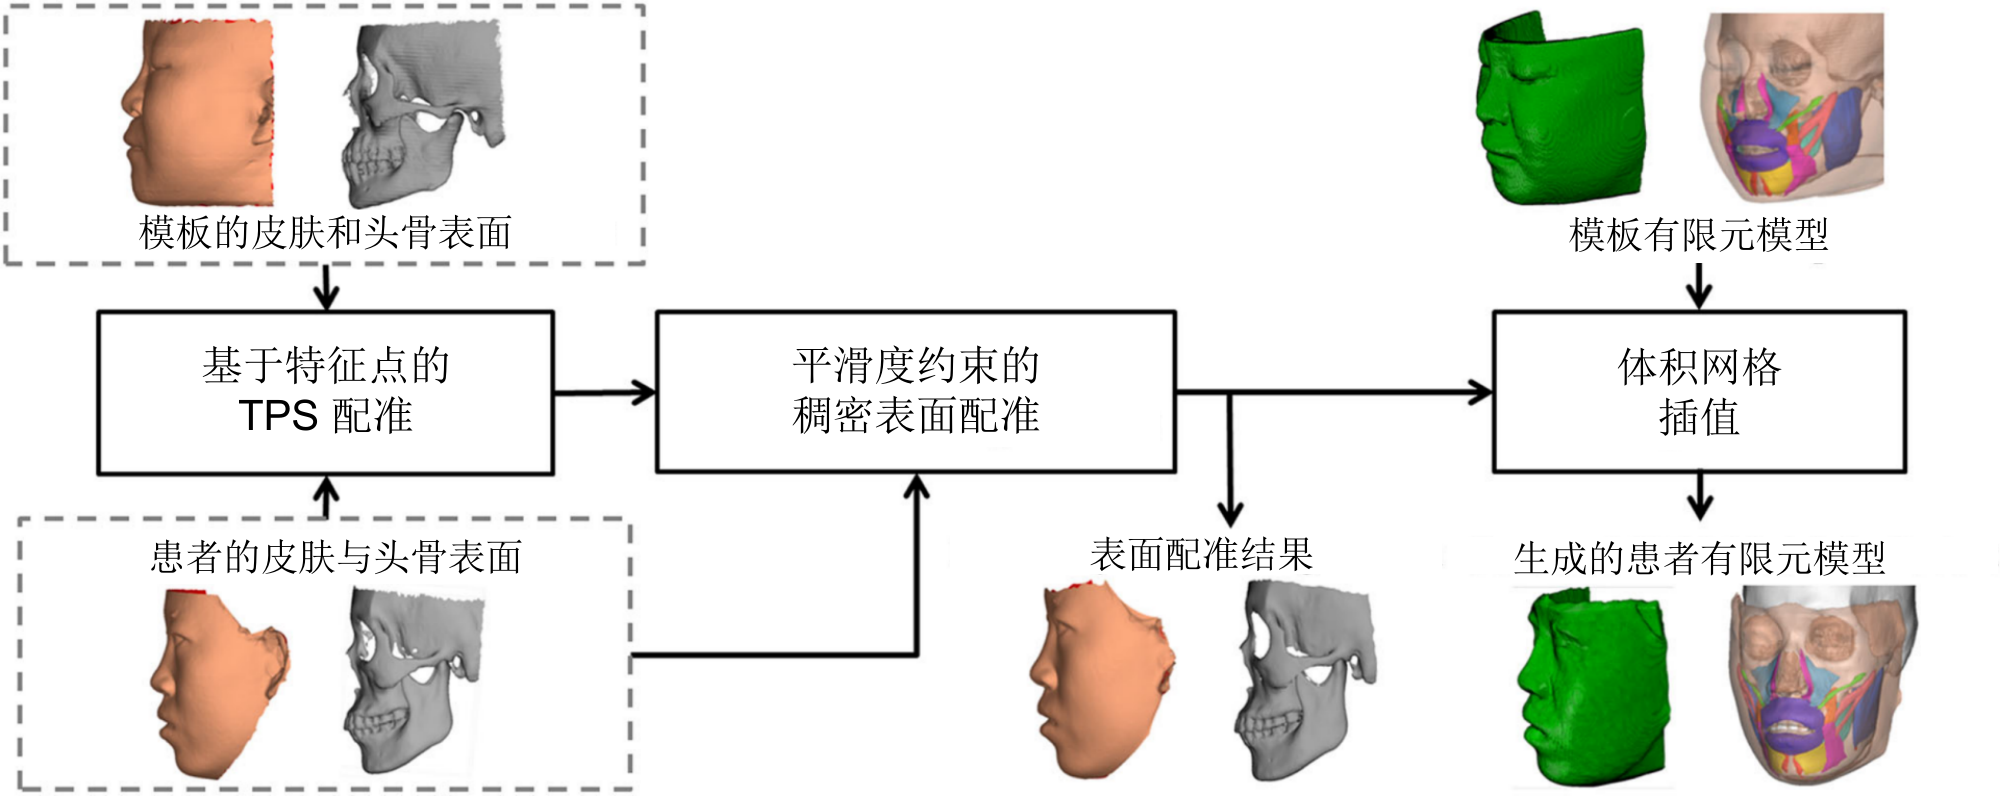
\includegraphics[width = \linewidth]{related-work/zhangEFacetemplateMethodEfficiently2016-cn.png}
  \caption{eFace-Template 技术框架 \cite{zhangEFacetemplateMethodEfficiently2016}}
  \label{fig:zhangEFacetemplateMethodEfficiently2016}
\end{figure}

\section{整形手术模拟研究进展}

在整形手术模拟领域,学术界已经进行了广泛而深入的研究。
目前,研究工作大致可以归结为两个主要方向:一是基于数据驱动的方法,这类方法使用先进的数据处理技术,以便预测整形手术的效果;另一方向是基于生物力学原理的仿真技术,该类技术利用计算机模型来精确预测手术后的结果。

\subsection{数据驱动的方法}

在计算机视觉的研究领域中,Zesong Qiu 等研究员 \cite{qiuSCULPTORSkeletonconsistentFace2022a} 提出了一个颇具创新性的三维参数化面部模型,被称为 SCULPTOR,其独特之处在于模型能够表达人类的骨骼结构。SCULPTOR 模型以 LUCY 数据集作为基础,将面部模型按不同维度进行解构,这些维度包括形状、姿态、表情等,从而构建了一种混合形状的表达形式。
该模型的核心在于以参数化方法驱动,集成了人类头骨结构、面部几何形状的建模,能够精确地捕获面部特征以及其背后的骨架结构。
特别是模型中引入的 trait 分量,对于模拟骨骼结构变化所引起的面部特征改变至关重要,这对于精确预测正颌手术患者术后面部外观的变化具有非常关键的意义。

\begin{figure}
  \centering
  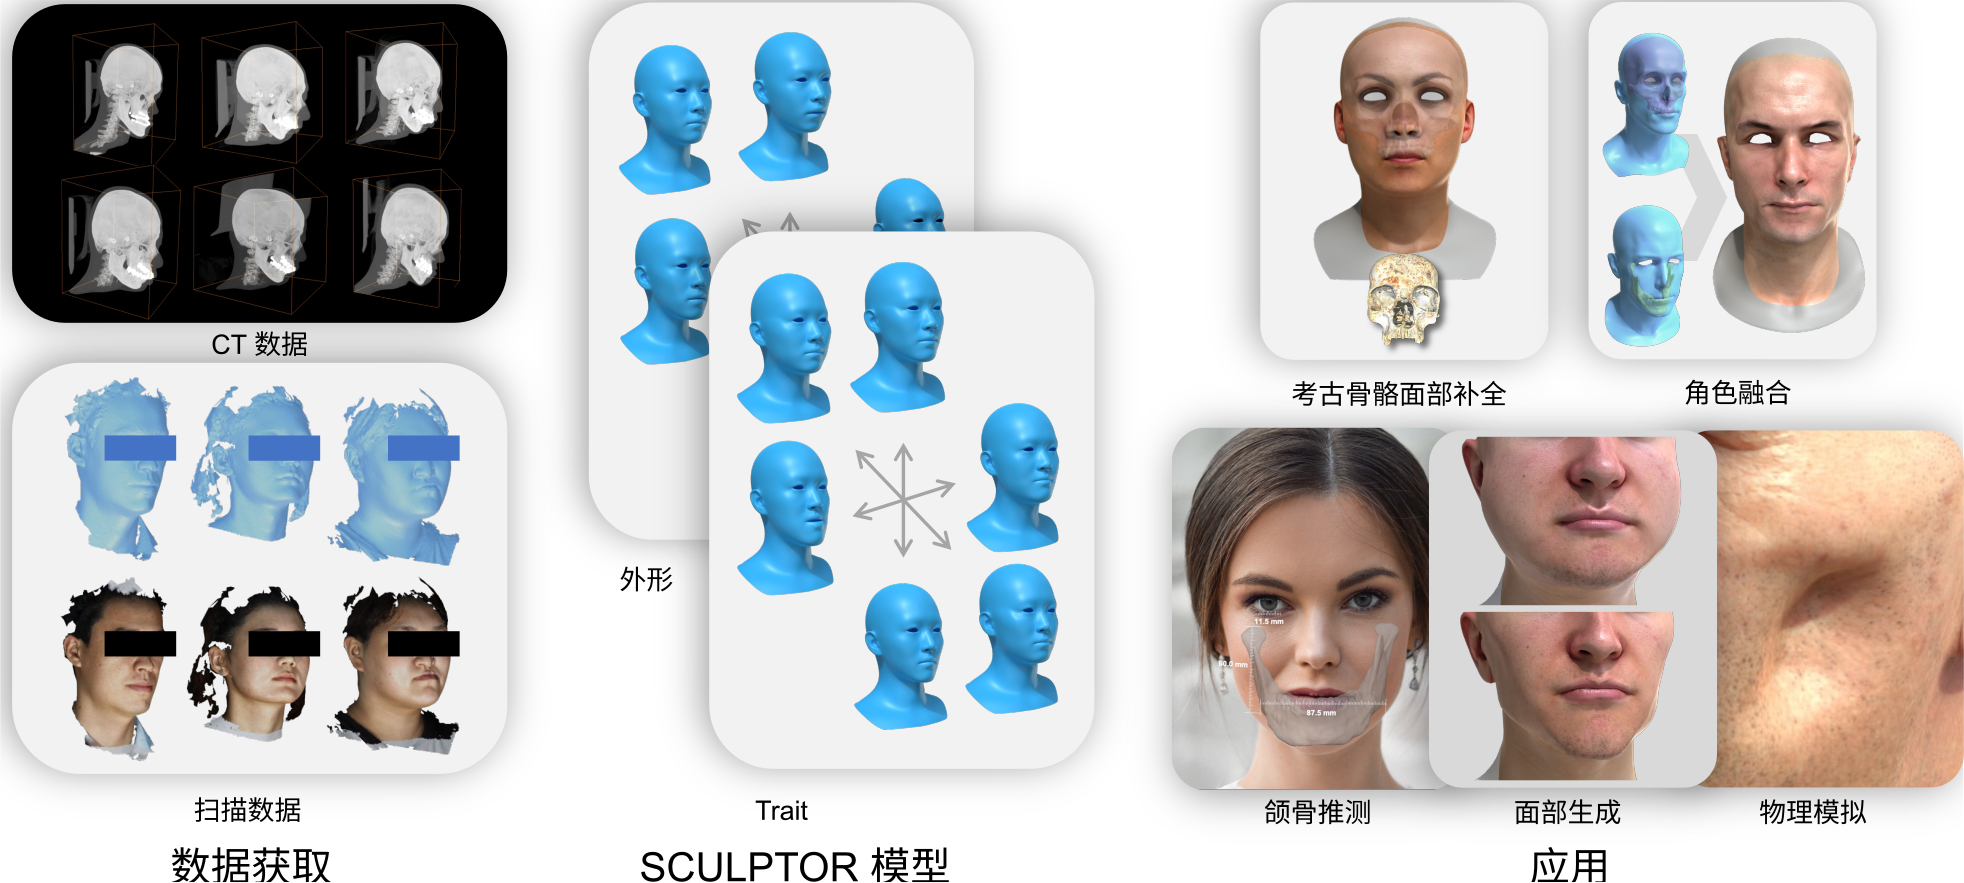
\includegraphics[width = \linewidth]{related-work/qiuSCULPTORSkeletonconsistentFace2022a-cn.png}
  \caption{SCULPTOR 模型概览 \cite{qiuSCULPTORSkeletonconsistentFace2022a}}
  \label{fig:qiuSCULPTORSkeletonconsistentFace2022a}
\end{figure}

在计算机视觉的研究领域内,深度学习技术已经取得了令人瞩目的成就,尤其在图像分类、目标检测和语义分割等任务上有卓越的表现。
近年来,众多研究者也开始探索将此技术应用于手术模拟的可能性。
Ma Lei 等研究人员 \cite{maSimulationPostoperativeFacial2023} 开发出一种称为 FSC-Net 的新型面部模型预测网络。
FSC-Net 的框架如图 \ref{fig:maBidirectionalPredictionFacial2023} 所示,该网络旨在学习从骨骼形态变化到面部外形变化之间的复杂且非线性的关系。
值得注意的是,FSC-Net 基于点变换网络结构,采用术前后成对数据进行弱监督学习来优化网络参数,这一过程无需严格的顶点对应匹配。
同时,为了提高建模的准确性,尤其是下颌部位,网络采用了以距离为基础的形状损失函数。
为了保持网格顶点的一致性并避免尖锐或不切实际的变形,FSC-Net 对顶点位移进行约束,以计算局部顶点损失。
实验评估显示,FSC-Net 在处理速度上比传统的有限元方法提高了 15 倍,同时还保持了与有限元方法相近的精度。

\begin{figure}
  \centering
  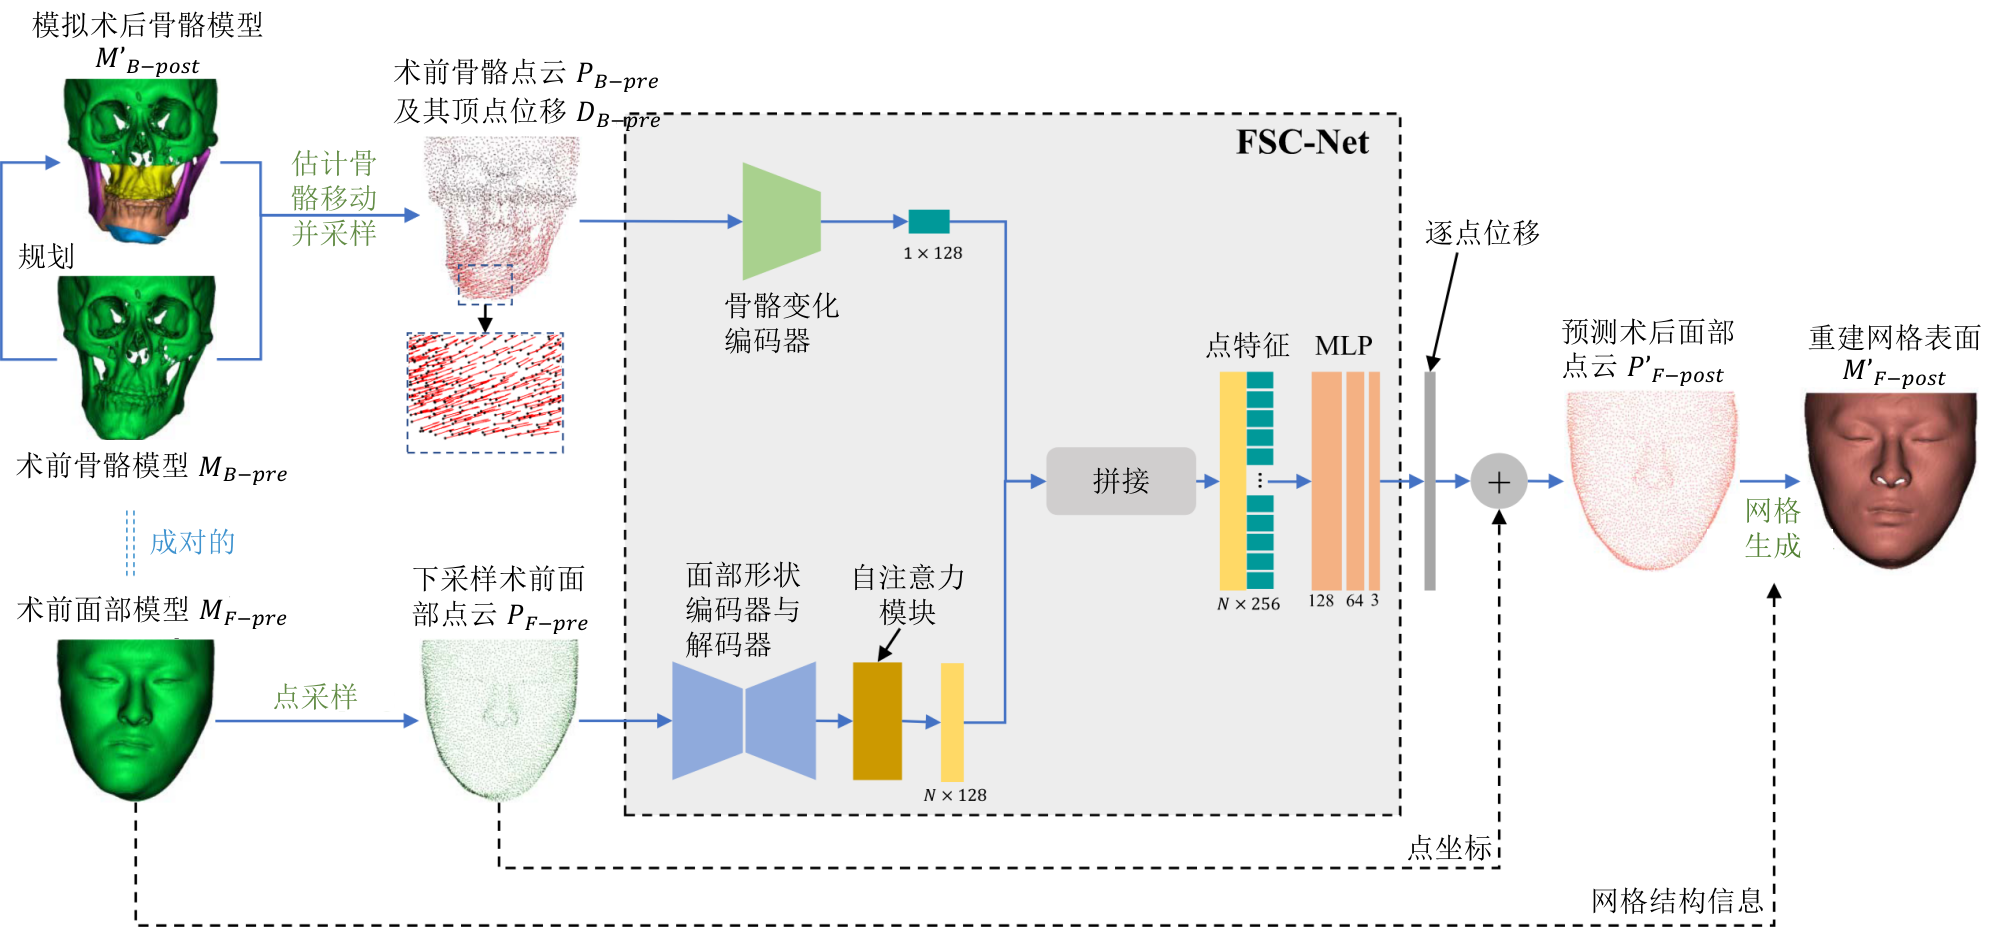
\includegraphics[width = \linewidth]{related-work/maSimulationPostoperativeFacial2023-cn.png}
  \caption{
    FSC-Net 框架概述 \cite{maBidirectionalPredictionFacial2023}
    % 。N:降采样后术前面部点云中的点数。MLP:多层感知器。
  }
  \label{fig:maBidirectionalPredictionFacial2023}
\end{figure}

在近一步的研究中,Ma Lei 等学者 \cite{maBidirectionalPredictionFacial2023} 在 P2P-Net \cite{yinP2PNETBidirectionalPoint2018} 的基础上进行了扩展,开发了一种新型深度学习模型,称为双向点对点卷积网络(P2P-Conv)。
这一模型专为解决面部和颅骨之间形态转换的问题而设计,旨在协助正颌外科手术规划。
P2P-Conv 不仅保留了 P2P-Net 的优势,还整合了动态点卷积(PointConv)技术,有效地提取了局部和全局空间信息。
模型训练时,该框架采用了多子集数据增广技术,通过分割面部和颅骨顶点为多个子集数据来增强训练过程。
在推理阶段,结合多子集产生的结果,可得到一致且精确的密集顶点变换预测。
实验结果表明,P2P-Conv 在面部和颅骨形态互换的预测准确性上取得了显著的进步。
然而,目前的方法还未能充分考虑到人体个体特异性这一问题 --- 例如,即便是颅骨形状极其相似的不同个体,他们的面部形态也可能存在显著的差异。

\subsection{物理仿真方法的研究进展}

关于面部软组织计算建模技术的研究已经吸引了广泛的关注,并取得了一系列深入的成果。
根据使用的建模方法不同,这些研究大致可以分为三大类:质点-弹簧模型(Mass Spring Model,MSM)、有限元模型(Finite Element Model,FEM)及质点-张量模型(Mass Tensor Model,MTM)。

在这三种模型中,由于计算效率上的显著优势,MSM 常被应用于实时面部动画制作。
Terzopoulos \cite{terzopoulosPhysicallyBasedFacial1990} 以及 Lee \cite{leeRealisticModelingFacial1995} 在该领域起到了开拓性的作用,他们开发的基于线性弹性肌肉的 MSM 能够高效地模拟面部动画。
此外,Keeve 等研究者 \cite{keeveDeformableModelingFacial1998} 提出了采用棱柱单元的 MSM,并针对精确度与计算成本,与有限元方法(FEM)进行了比较分析。

经过深入研究,Teschner 等学者 \cite{teschnerDirectComputationNonlinear} 提出了一种改进的多层非线性 MSM,该方法通过引入静态约束来直接计算面部模拟仿真中的平衡状态。
Vicente \cite{vicenteMaxillofacialSurgerySimulation2009} 的工作专注于利用 MSM 技术模拟面部手术后的形态变化,创新性地设计了基于六面体元素网格的 MSM。
这个模型在理论上与传统线性 FEM 等价,并通过位移尺度调整技术细致模拟软组织的物理响应。

与传统的 MSM 对比,FEM 在模拟生物力学特性方面具有更高准确性,尽管其计算相对更加耗时。
Kim 等研究者 \cite{kimClinicallyValidatedPrediction2017} 提出了一种新颖的三阶段有限元方法,通过模拟组织之间的滑动来增强面部软组织变形预测的精确度。
在第一阶段,该方法利用 eFace-Template \cite{zhangEFacetemplateMethodEfficiently2016} 构造患者的网格模型,并以手术后骨骼的位移作为边界条件,应用 FEM 模拟软组织响应。
第二阶段引入节点力约束来仿真软组织与骨骼之间的滑动效应,显著提升了模拟结果的质量。
最后,在第三阶段通过重构软组织与骨骼间的映射关系,并引入新的节点间空间约束作为边界条件,进一步增强模拟组织滑移效应的仿真质量。
研究表明,这种改良的 FEM 在模拟面部结构,特别是在临床关键区域如鼻子和口唇的精确度方面,相较于现有的其他 FEM 技术有明显提高。

为了精确预测面部软组织术后的位置变化,Knoops等研究者 \cite{knoopsNovelSoftTissue2018} 开发了创新的概率有限元模型。
该模型结合了实验设计方法(Design Of Experiments,DOE)与迭代优化策略,成功地生成了一系列具有概率预测区间的三维面部模型,特别是针对鼻部和上唇区域,展现出高度的预测准确性。
此项研究深入剖析了模型的不准确性和手术计划执行中的不确定性对软组织预测结果的影响。
此外,该模型为手术规划提供了可能的区间预测,对于帮助患者充分了解手术可能引起的面部变化具有重要的临床意义。

在数值模拟领域,MTM 的设计宗旨是实现计算效率与结果精度之间的优化平衡。
开拓性研究者 Cotin 等人 \cite{cotinHybridElasticModel2000} 率先提出了一种基于 MTM 的混合弹性模型,该模型致力于精确描绘软组织在局部变形时表现出的复杂物理效应。
在此基础上,Picinbono 及其研究伙伴 \cite{picinbonoNonlinearAnisotropicElasticity2003} 进一步发展了这一模型,将其应用到非线性各向异性材料的相关研究中。

Mollemans 的研究团队 \cite{mollemansPredictingSoftTissue2007} 创新性地将 MTM 技术应用于颅颌面手术的软组织模拟中,通过对临床案例的定量与定性评估,首次实地验证了该技术在此类应用中的可靠性和有效性。
此后,Kim 等研究者 \cite{kimNewSofttissueSimulation2010} 使用了横向各向同性的 MTM,探索如何进行面部软组织行为的预测,并提出了一种同时满足生物力学原理与高效率仿真需求的软组织模拟方法。

在类似研究的进一步深化中,Ichim 及其同事 \cite{ichimPhacePhysicsbasedFace2017} 创新性地提出了 Phace --- 这是一种基于物理原理的面部动画技术。
Phace 建立在一个精心构建的通用面部模板之上,如图 \ref{fig:ichimPhacePhysicsbasedFace2017} 所示,其中包含了组织和骨骼的体积表示、嵌入四面体网格的肌肉模型、一组混合形状基等信息。
与传统的模拟方法不同,Phace 通过最小化被动肌肉、主动肌肉与骨骼这些刚体结构交互作用过程中的势能,实现对于面部表情动态变化的精确计算。
而且,Phace 通过将碰撞处理机制与仿真模型整合,有效规避了传统动画技术如混合形状建模中常见的穿模问题。
通过引入的全新肌肉激活模型,Phace 能够有效地复现复杂的面部表情。
Phace 所展现出的应用潜力极为广泛,它不仅适合于艺术动画制作的场景,还可服务于模拟整形手术过程中的面部重塑以及脸部与外力或物体相互作用的动态模拟。

\begin{figure}
  \centering
  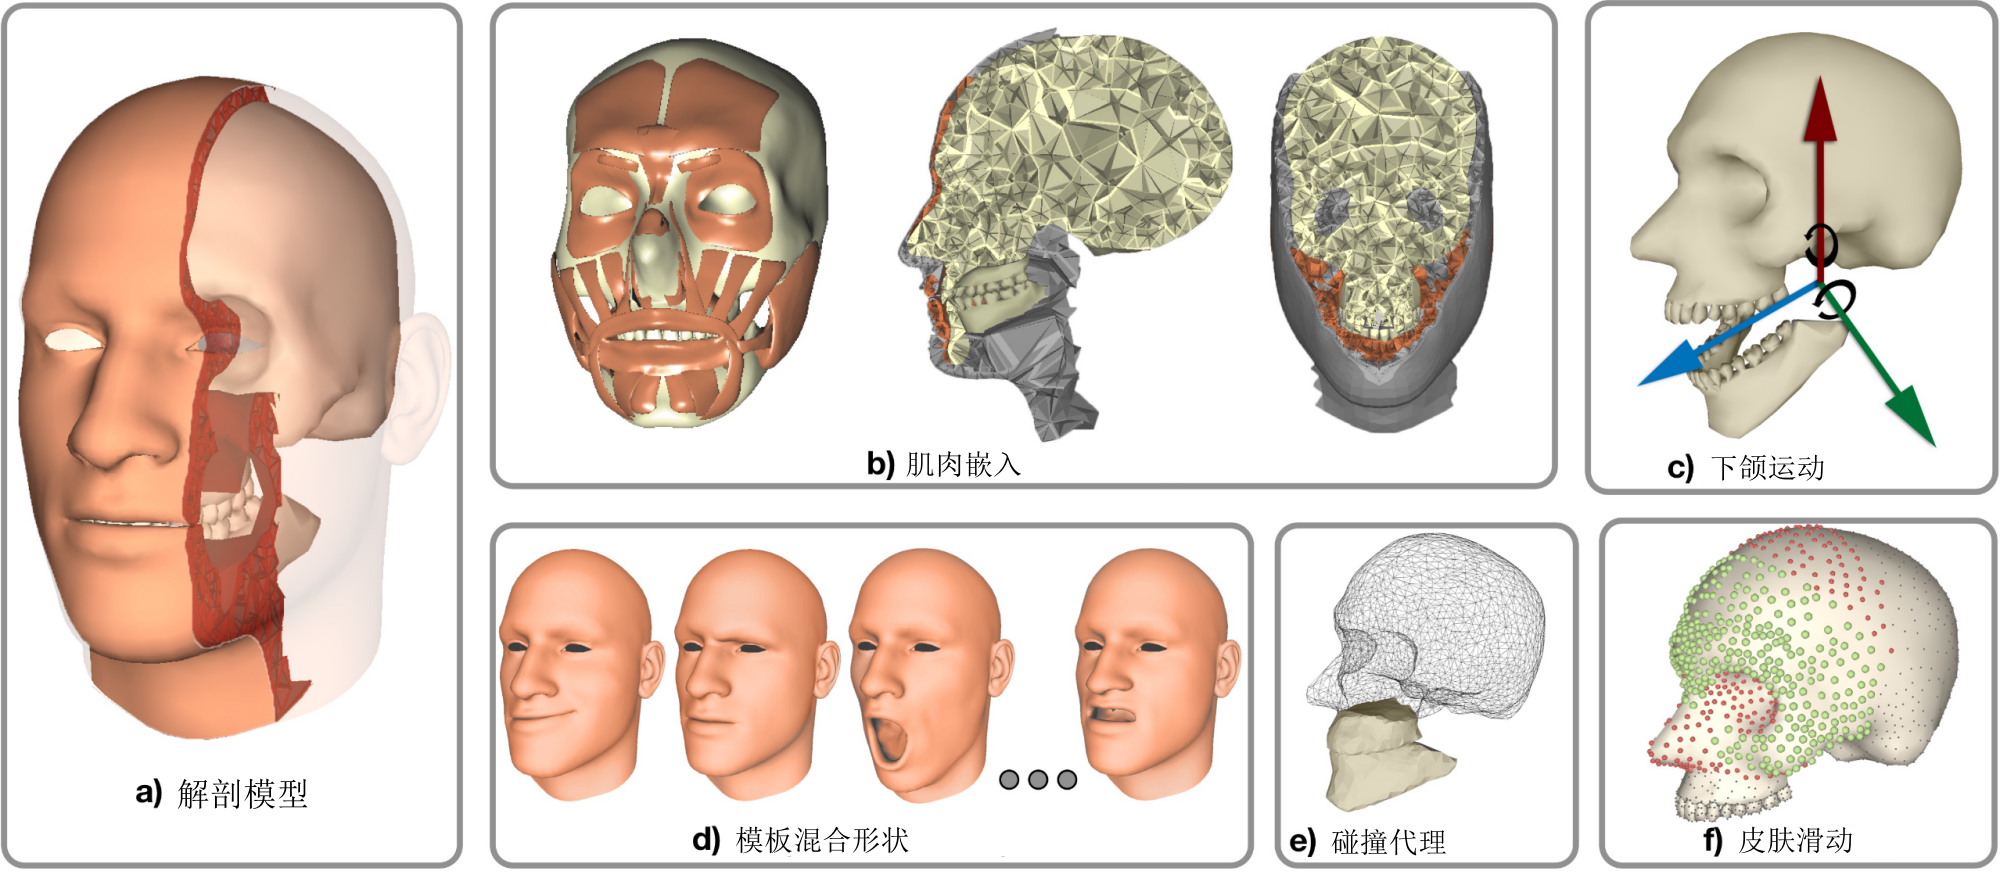
\includegraphics[width = \linewidth]{related-work/ichimPhacePhysicsbasedFace2017-cn.png}
  \caption{Phace 模板构成 \cite{ichimPhacePhysicsbasedFace2017}}
  \label{fig:ichimPhacePhysicsbasedFace2017}
\end{figure}
